\section{Le fratture}

\subsection{Introduzione}

Le fratture sono definite come delle \emph{soluzioni di continuità di un segmento osseo}.

Ogni segmento osseo ha una sua resistenza: per generare una frattura quindi l'entità del trauma deve superare i limiti di elasticità e di resistenza del segmento osseo colpito.

Di fronte ad una frattura (ad esempio di un osso lungo come il femore) si possono riconoscere:

\begin{itemize}
\item
  \textbf{Focolaio di frattura:} corrisponde alla sede anatomica della frattura
\item
  \textbf{Rima della frattura:} rappresenta l'andamento della linea di demarcazione fra due o più segmenti di osso fratturato
\item
  \textbf{Monconi della frattura:} segmenti principali dell'osso fratturato
\end{itemize}

\begin{figure}[!ht]
\centering
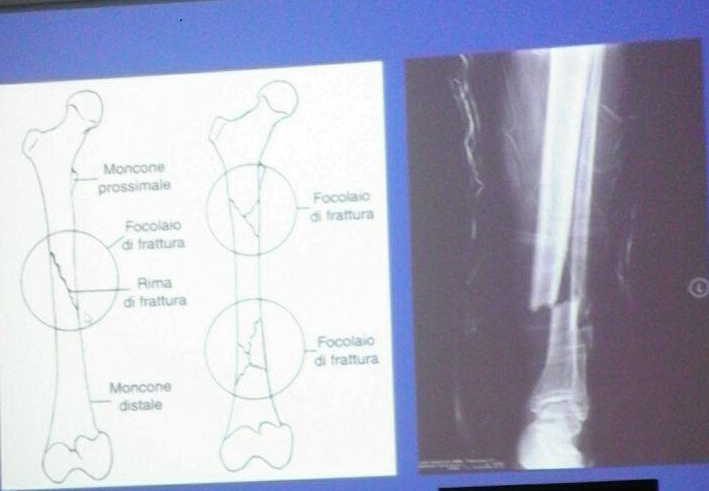
\includegraphics[width=0.9\textwidth]{002/image1.png}
\end{figure}


\subsection{Classificazione}

Le fratture possono essere classificate secondo diversi criteri.

\subsubsection{I. CLASSIFICAZIONE EZIOLOGIA} 
(è la classificazione più utilizzata) Dal punto di vista eziologico distinguiamo:

\begin{figure}[!ht]
\centering
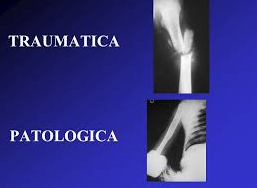
\includegraphics[width=0.7\textwidth]{002/image2.png}
\end{figure}

\paragraph{Fratture traumatiche}
Sono le fratture più frequenti e si verificano quando \emph{un \textbf{unico trauma efficiente} causa l'interruzione di un osso sano e strutturalmente normale.} Ad esempio se un motociclista urta contro un palo con conseguente frattura di tibia e perone allora definiremo quella come una frattura traumatica legata al trauma diretto della gamba contro il palo.

\paragraph{Fratture da durata o da stress}
Conseguenti \emph{a ripetuti \textbf{microtraumi non efficienti} che agiscono nel tempo su un osso sano}. Il cedimento strutturale è \emph{per sovraccarichi funzionali che superano i limiti di resistenza meccanica dell'osso stesso. Sono per definizione stessa delle fratture incomplete! Tuttavia se il meccanismo lesivo non viene interrotto, evolvono in vere e proprie fratture complete che coinvolgono principalmente gli arti inferiore dal momento che questi sono esposti a carichi di lavoro maggiori.} Possiamo prendere in considerazione diverse situazioni come ad esempio quella di un maratoneta che si allena costantemente e partecipa a 3/4 maratone l'anno, può andare incontro ad una frattura da stress del metatarso. Altra frattura da stress comune è quella dei metacarpi nei pugili o del collo del femore o del piatto tibiale nei Marines (c'è molta letteratura al riguardo).

\paragraph{Fratture patologiche}
Si tratta di una tipologia la cui incidenza è progressivamente aumentata negli ultimi anni. Si instaurano su un \emph{``osso patologico}'' cioè un osso che risulta essere più debole del normale e meccanicamente insufficiente. Molto spesso non è nemmeno presente l'evento traumatico o talvolta è un trauma inefficace. Le cause che portano ad un indebolimento dell'osso possono essere varie e ne vediamo alcune:

\subparagraph{Osteoporosi}
Ad esempio una persona anziana che si alza dalla sedia e accusa poi dolore alla schiena, può riportare una frattura dei corpi vertebrali su base osteoporotica. \emph{L'osteoporosi è definita come una riduzione della massa ossea con rarefazione delle trabecole nell'osso spongioso e assottigliamento della corticale che comporta un aumentato rischio di fratture. Va sottolineato che nell'osteoporosi la massa ossea è quantitativamente ridotta, ma qualitativamente normale perciò possono verificarsi fratture per traumi molto modesti come ad esempio al collo del femore o alle vertebre e nella maggior parte dei casi sono conseguenti a traumi multipli piuttosto che ad un unico trauma evidente.}
\textbf{N.B.:} Non abbiamo una definizione univoca per le fratture da osteoporosi. Sul libro dice chiaramente che non sono classificabili come fratture patologiche, ma nella lezione sulle fratture del collo del femore (sulla vecchia dispensa Sigfied) il prof Ceccarelli le inserisce tra le fratture patologiche ``border-line''. Durante questa lezione (tenuta dal prof. Vaienti) sono riportate come esempio di fratture patologiche e chiesti chiarimenti al prof., questi ribadisce che loro le considerano come patologiche!

\subparagraph{Malattie congenite}
Come ad esempio l'osteogenesi imperfetta (OI). \emph{Detta anche malattia delle ossa di vetro o malattie delle sclere blu, l'OI è una patologia che colpisce gli individui di sesso maschile principalmente ed è dovuta ad anomalie nella sintesi del collagene di tipo I con problemi a carico dello scheletro, delle articolazione, degli occhi (sclere blu), delle orecchie, della cute e dei denti. Può essere a penetranza più o meno completa e, conseguentemente, ad espressione clinica più o meno grave: oggi se ne conoscono sette tipologie a gravità diversa.}

\subparagraph{Tumori}
Sia tumori primitivi alle ossa come cisti ossee o tumori maligni primitivi sia metastasi di tumori in altre sedi tra cui più frequentemente tumore della mammella, del polmone, della prostata e dell'utero. \emph{Questi possono colpire tanto i bambini quanto gli adulti però nei bambini sono generalmente più benigni.}

\subparagraph{Infezioni}
Come nel caso dell'osteomielite
\\\\
N.B.Delle cause riportate ricordare che l'osteogenesi imperfetta è la causa più ricorrente tra i bambini mentre l'osteoporosi tra gli anziani.
Le lesioni osteolitiche di natura neoplastica benigne o maligne, primitive o secondarie riguardano principalmente gli adulti e anziano, ma a volte anche i bambini


\paragraph{Fratture iatrogene o osteotomie chirurgiche}
Interruzioni del tessuto osseo \emph{realizzate dal chirurgo a fini terapeutici quindi per correggere una deformità.} Possono essere realizzate manualmente o più frequentemente mediante l'utilizzo di strumenti chirurgici (seghe, fili, scalpelli, osteotomi). Ad esempio nel caso di ginocchio varo (è il cosiddetto ginocchio a parentesi: l'opposto del ginocchio a X o ginocchio valgo) viene trattato schematicamente così: con lo scalpello si effettua la frattura iatrogena quindi si corregge la deformità ed infine si blocca il tutto con una piastra e delle viti. Per l'osteotomia dell'anca finalizzata a correggere un'anca displasica (es. osteotomia di Salter, osteotomia di Chiari) si procede come di seguito: si frattura l'acetabolo, si riorienta nella posizione corretta e poi si blocca con delle viti. \emph{Infine l'osteotomia è eseguita anche per correggere eterometrie degli arti.} \emph{La calloclasia invece è l'interruzione chirurgica di un callo osseo che si effettua quando la frattura si sta riparando in modo inadeguato}


\begin{figure}[!ht]
\centering
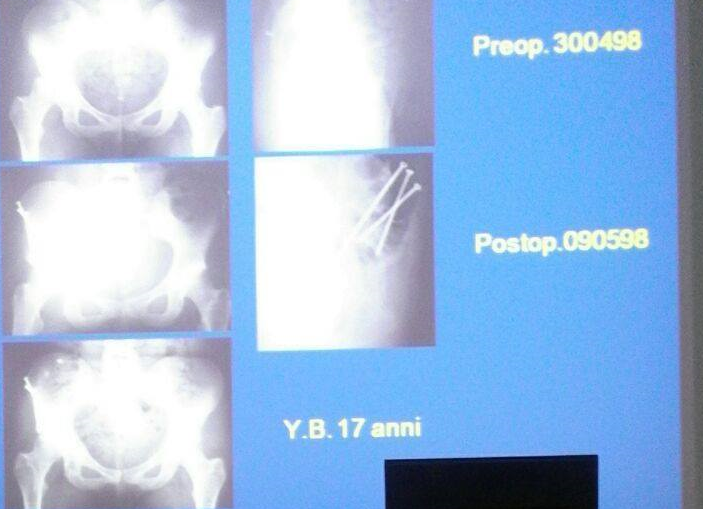
\includegraphics[width=0.7\textwidth]{002/image3.png}
\end{figure}


\subsubsection{II. CLASSIFICAZIONE IN BASE AL TIPO DI TRAUMA}

\paragraph{Frattura per trauma diretto}
Il trauma agisce nel punto stesso in cui si manifesta la frattura. Ad esempio un soggetto che riceva un calcio al terzo medio della tibia con conseguente frattura dell'osso in quel punto. \emph{Distingueremo in questo caso:}

\begin{itemize}
\item
  \emph{Fratture da urto}
\item
  \emph{Fratture da schiacciamento}
\item
  \emph{Fratture penetranti (o da arma da fuoco)}
\end{itemize}

\paragraph{Frattura per trauma indiretto}
In questo caso il trauma causa una frattura a distanza rispetto al punto di applicazione del trauma stesso. Ad esempio chi cade sulla mano, ma riporta una frattura del gomito. \emph{{[}La vecchia dispensa Sigfied suddivide ulteriormente la fratture indirette in fratture per torsione, per flessione, per compressione, per trazione e per azione combinata. Nella lezione il prof non riporta tale sub classificazione e procede con la classificazione in base al meccanismo lesivo che coincide con tale sub classificazione riportata nella vecchia dispensa{]}}


\subsubsection{III. CLASSIFICAZIONE IN BASE AL MECCANISMO LESIVO}

\paragraph{Fratture da flessione}
Il trauma determina una modifica della normale curvatura dell'osso fino alla rottura. \emph{Ad esempio le ginnaste che flettono troppo l'ulna.}
\paragraph{Fratture da torsione}
In questo caso il trauma è di tipo torcente rispetto all'asse osso. \emph{Ad esempio se metto il piede tra il marciapiede e un altro ostacolo, il piedi si incastrerà e cadrò in avanti: si produce una rima di frattura spiroide.}
\paragraph{Fratture da compressione o da schiacciamento}
\emph{L'esempio tipico è a livello dell'osso spongioso vertebrale}
\paragraph{Fratture da strappamento}
In questo caso la trazione di un legamento o di un tendine causa il distacco dell'osso che ivi si inserisce\emph{.} Ad esempio a volte il legamento rotuleo ``strappa l'osso a livello della sua inserzione sulla tuberosità tibiale anteriore
\paragraph{Fratture per azione combinata}


\subsubsection{IV. CLASSIFICAZIONE IN BASE AL DECORSO DELLA RIMA}

\paragraph{Fratture trasversali}
La rima è ad \emph{angolo retto} rispetto all'asse longitudinale dell'osso
\paragraph{Fratture oblique}
La rima forma un \emph{angolo minore di 90\textsuperscript{o}} rispetto all'asse longitudinale
\paragraph{Fratture spiroidi}
La rima compie un \emph{decorso a spirale} rispetto al segmento osseo
\paragraph{Fratture longitudinali}
La rima è \emph{parallela} all'asse longitudinale dell'osso

\begin{figure}[!ht]
\centering
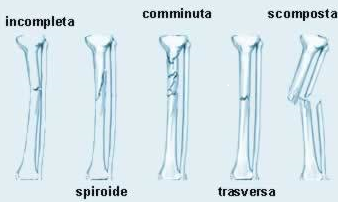
\includegraphics[width=0.7\textwidth]{002/image4.png}
\end{figure}

\begin{figure}[!ht]
\centering
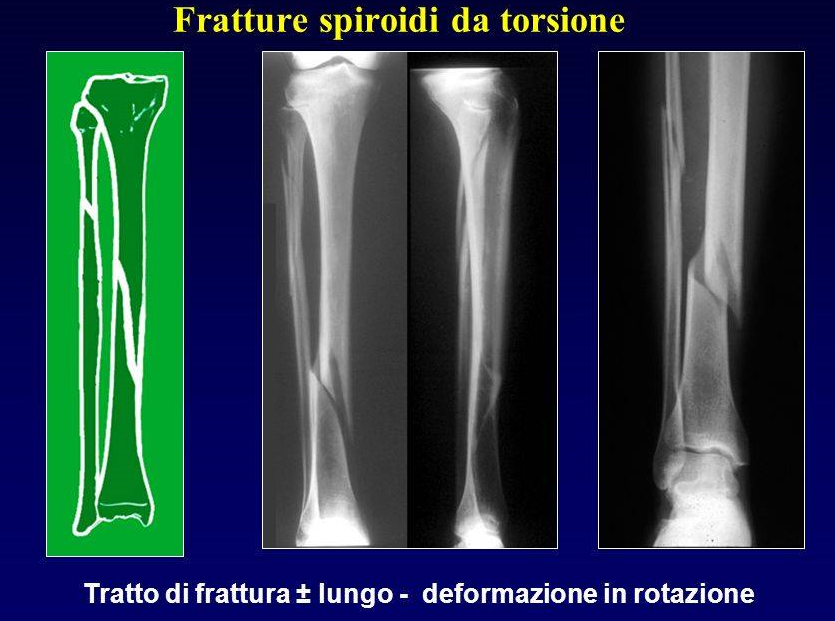
\includegraphics[width=0.7\textwidth]{002/image5.png}
\end{figure}


\subsubsection{V. CLASSIFICAZIONE PER SPOSTAMENTO DEI MONCONI}

\paragraph{Fratture composte}
I frammenti \emph{conservano} la loro posizione e rapporti anatomici \emph{così da non modificare la normale configurazione dell'osso.}
\paragraph{Fratture scomposte} 
I frammenti \emph{non conservano} la loro posizione anatomica \emph{e la forma del segmento scheletrico appare alterata dallo spostamento dei frammenti stessi. Per la diafisi delle ossa lunghe si descrivono 4 tipi di scomposizione}

\begin{itemize}
\item
  \emph{Longitudinale:} i monconi si sovrappongono in lunghezza l'uno sull'altro
\item
  \emph{Angolare:} i monconi si angolano l'uno rispetto all'altro
\item
  \emph{Laterale:} i monconi non si sovrappongono, ma sono spostati lateralmente l'uno rispetto all'altro
\item
  \emph{Rotatorio:} i monconi ruotano l'uno sull'altro
\end{itemize}

\paragraph{Fratture scomposte e ingranate} 
I monconi si ingranano l'uno sull'altro. Generalmente sono dovute a traumi da compressione. Una frattura scomposta ed ingranata dei corpi vertebrali, si riconosce all'RX perché normalmente il corpo vertebrale appare di forma rettangolare mentre in caso di frattura ingranata il rettangolo scompare e si vede una cuneizzazione perché la parte anteriore si schiaccia rispetto a quella posteriore

\begin{figure}[!ht]
\centering
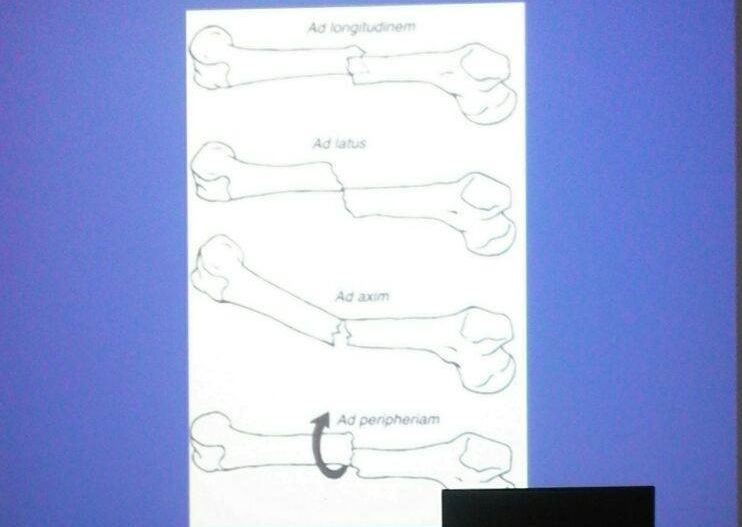
\includegraphics[width=0.7\textwidth]{002/image6.png}
\end{figure}


\subsubsection{VI. CLASSIFICAZIONE PER NUMERO DI FRAMMENTI}

\paragraph{Fratture unifocali}
Una rima di frattura e due monconi
\paragraph{Fratture bifocali} 
Due focolai di frattura posti a livelli diversi e tre monconi
\paragraph{Fratture plurifocali o pluriframmentarie} Tanti focolai di frattura e tanti monconi.


\subsubsection{VII. CLASSIFICAZIONE PER SEDE SCHELETRICHE (per ossa lunghe)}

\paragraph{Fratture diafisarie}
La diafisi è la parte centrale di un osso lungo
\paragraph{Fratture epifisarie} 
L'epifisi è la parte articolare distale di un osso lungo
\paragraph{Fratture metafisarie} 
La metafisi è a metà tra epifisi e diafisi


\subsubsection{VIII. CLASSIFICAZIONE PER ALTRA SEDE (no sede scheletrica!)}

È la classificazione più comunemente riportata nei referti:

\paragraph{Frattura articolare} 
\emph{La rima di frattura intacca la cartilagine articolare}. Caratterizzata da una prognosi peggiore legata alla maggiore frequenza di insorgenza di artrosi post-traumatica; per scongiurare tale evoluzione si cerca di ripristinare un piano cartilagineo il più normale possibile tuttavia molto spesso la cartilagine è troppo rovinata oppure risulta impossibile rimetterla a posto quindi si lasciano degli scalini di incongruenza.
\paragraph{Frattura extra-articolare} 
La rima di frattura non arriva a livello della cartilagine articolare e questo generalmente si associa ad una prognosi migliore perché non c'è rischio di artrosi post-traumatica. \emph{Queste sono ulteriormente suddivise in:}

\begin{itemize}
\item
  \emph{Intra-capsulari: sono generalmente piuttosto gravi perché spesso vanno incontro a devascolarizzazione e il danno vascolare limita la capacità di creare un callo osseo}
\item
  \emph{Extra- capsulari}
\end{itemize}

\begin{figure}[!ht]
\centering
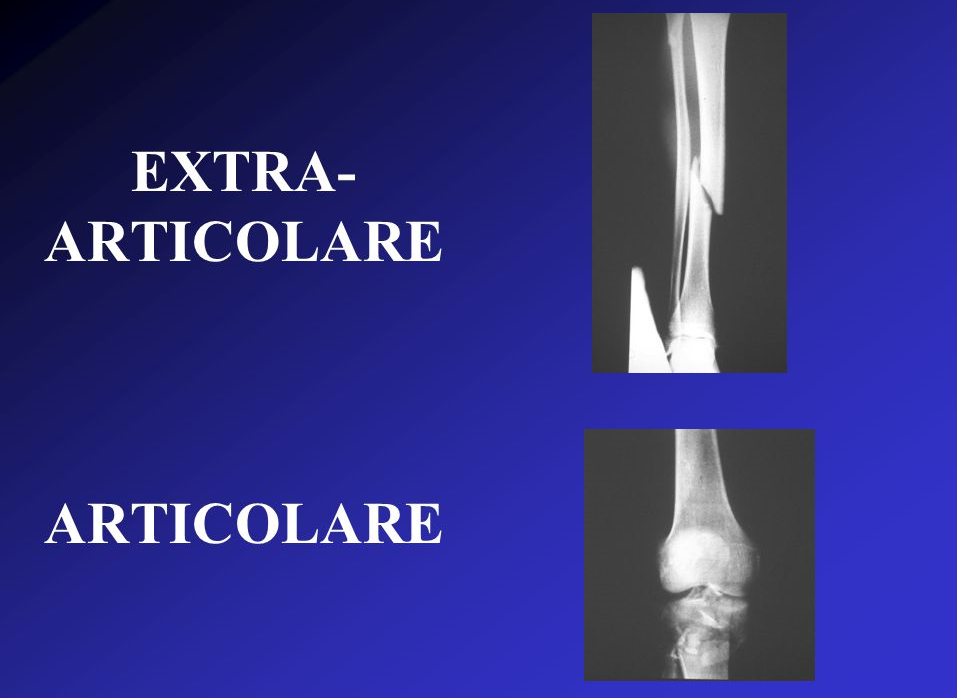
\includegraphics[width=0.7\textwidth]{002/image7.png}
\end{figure}

\subsubsection{IX. CLASSIFICAZIONE PER ENTITA' DEL DANNO}

\paragraph{Fratture complete}
Interessano \emph{tutta la circonferenza} dell'osso
\paragraph{Fratture incomplete} 
\emph{Non} interessano tutta la circonferenza. Possono essere a loro volta ulteriormente suddivise in:

\begin{itemize}
\item
  Fratture per infrazione
\item
  Fratture ``a legno verde'': questa espressione viene generalmente utilizzata quando si è di fronte ad una frattura in un bambino poiché in questo caso le loro ossa lunghe sono più plastiche rispetto a quelle di un adulto e quindi sono esposte ad un minor rischio di frattura. In questo caso avremo uno sfibramento o una piegatura, ma non una rottura dell'osso da cui il paragone con il legno verde che ha bisogno di una stimolazione più forte per spezzarsi rispetto ad un legno secco.
\end{itemize}


\begin{figure}[!ht]
\centering
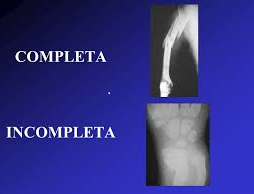
\includegraphics[width=0.7\textwidth]{002/image8.png}
\end{figure}

\subsubsection{X. CLASSIFICAZIONE IN BASE ALL'INTEGRITA' DEL MANTELLO CUTANEO}

Si tratta di una classificazione molto importante per gli ortopedici

\begin{figure}[!ht]
\centering
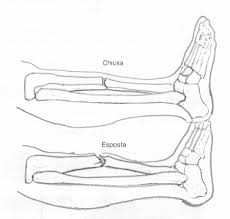
\includegraphics[width=0.5\textwidth]{002/image9.png}
\end{figure}

\paragraph{CHIUSE}
Attorno alla rima di frattura e ai monconi \emph{la cute è integra}
\paragraph{ESPOSTE (O APERTE)}
\emph{L'integrità cutanea è interrotta} e il focolaio di frattura comunica con l'ambiente esterno tramite una ferita più o meno ampia. \emph{In questo caso il focolaio della frattura è esposto a contaminazione microbica che può evolvere verso una vera e propria osteomielite.} Sono molto importanti perché rappresentano delle urgenze chirurgiche.

\begin{figure}[!ht]
\centering
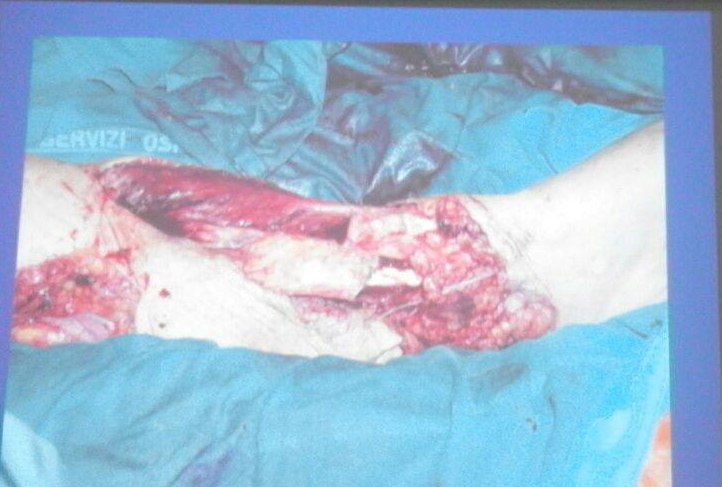
\includegraphics[width=0.5\textwidth]{002/image10.png}
\end{figure}

\subsection{Urgenze}

\begin{itemize}
\item
  \textbf{Fratture esposte}: devono essere portate in sala operatoria massimo entro 6/8 ore (tempo minimo oltre il quale può insorgere infezione. L'infezione all'osso è difficilissima da trattare perché l'osso è già di per sé un tessuto a cui arriva poco sangue e in uno danneggiato ne arriva ancora meno). Nel minor tempo possibile l'ortopedico deve pulire il focolaio, rimuovere i tessuti necrotici, stabilizzare con un fissatore a ponte e coprire il più possibile con muscoli, sottocute e cute la ferita.
\item
  \textbf{Distacchi epifisari}: parliamo di distacco epifisario quando, nei bambini e nei giovani adulti, si osserva la separazione traumatica dell'epifisi dalla metafasi alla quale aderisce per interposizione della cartilagine di accrescimento (la rima di frattura passa attraverso la cartilagine di accrescimento). Ricordate che il tessuto cartilagineo fertile guida l'accrescimento delle ossa lunghe. Possono essere distinti in:

\begin{itemize}
\item
  \textbf{Puri}: è interessata \emph{solo} la cartilagine di accrescimento.
\item
  \textbf{Misti:} la rima di frattura di estende al tessuto contiguo perciò sono interessate la cartilagine di accrescimento e la cartilagine sopra e/o sottostante.
\end{itemize}

Anche queste devono essere stabilizzate entro 6/8 ore,
l\textbf{'}obiettivo è quello di agire il prima possibile per evitare la morte delle cellule della zona di accrescimento. Non è prevedibile se l'accrescimento avverrà poi in maniera normale oppure no, con i genitori bisogna essere sempre molto schietti e diretti: si vedrà nel tempo cosa
accadrà.

\begin{figure}[!ht]
\centering
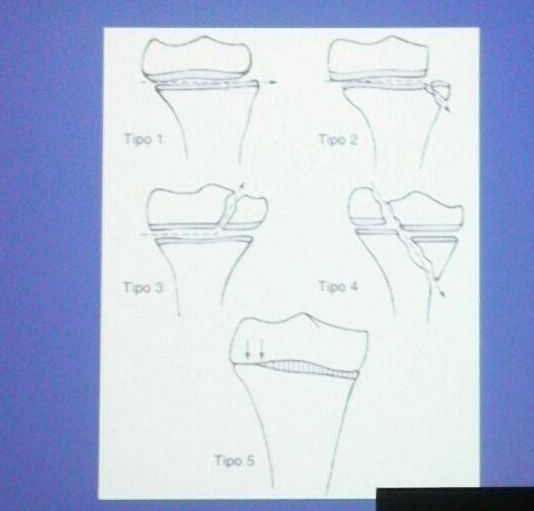
\includegraphics[width=0.5\textwidth]{002/image11.png}
\end{figure}

\emph{La classificazione di Salter- Harris prevede la distinzione dei distacchi epifisari in 5 tipi, in rapporto al decorso della rima di frattura}

\begin{figure}[!ht]
\centering
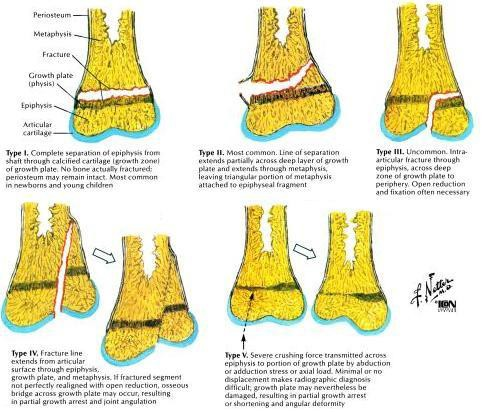
\includegraphics[width=0.7\textwidth]{002/image12.jpeg}
\end{figure}

Possibili inconvenienze in caso di distacchi epifisari possono essere:

\begin{itemize}
\item
  Ipometria (un arto cresce meno dell'altro)
\item
  Distorcimento (un arto cresce storto)
\end{itemize}

\item
  \textbf{Frattura-Lussazione}: Definiamo la lussazione come una perdita \emph{permanente} dei rapporti tra due capi articolari (il classico esempio è quando un soggetto cade e si ha lussazione della spalla: si dice che la spalla ``esce'' e non si riesce a ``rimetterla dentro''). La lussazione è da differenziare invece dalla distorsione definita come una perdita \emph{temporanea} dei rapporti tra due capi articolari.

Le lussazioni sono delle emergenze e devono essere trattate applicando una trazione per rimettere a posto i capi articolari. Quando siamo di fronte ad una lussazione prima di fare qualsiasi manovra dobbiamo sempre eseguire un RX per valutare la possibilità che ci sia anche una frattura. L'RX va sempre eseguita anche dopo la manovra di trazione.

\end{itemize}


\subsection{Diagnosi}

Di fronte ad un sospetto clinico di frattura bisogna fare una diagnosi: in prima battuta una diagnosi clinica che dovrà poi essere confermata con delle indagini strumentali.

\textbf{Diagnosi clinica}:

Di fronte ad un sospetto di frattura avremo:

\begin{itemize}
\item
  \textbf{Segni di probabilità}

\begin{itemize}
\item
  \emph{Atteggiamento} ad esempio l'extra-rotazione e accorciamento della gamba indicano una possibile frattura del femore
\item
  \emph{Deformità} ad esempio il dorso a forchetta nella frattura di polso

\begin{figure}[!ht]
\centering
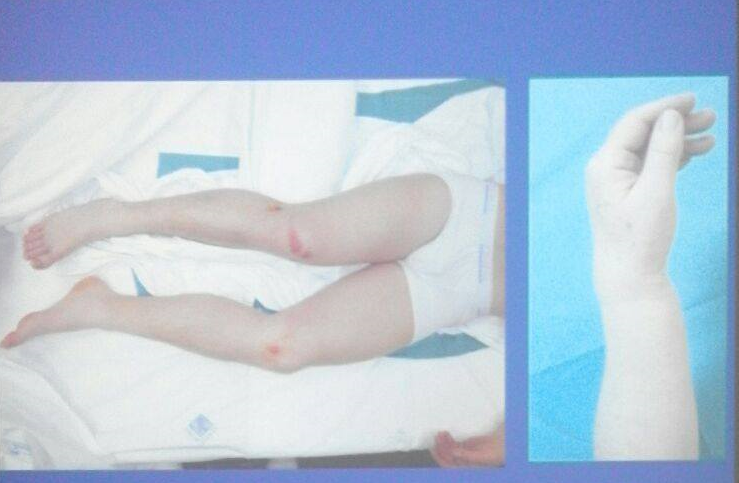
\includegraphics[width=0.7\textwidth]{002/image13.png}
\end{figure}

\item
  \emph{Ferite/ecchimosi}
\item
  \emph{Tumefazioni e lesioni cutanee}
\item
  \emph{Dolore importante}
\item
  \emph{Impotenza funzionale} ad esempio il paziente non riesce a muovere l'arto interessato o a camminare
\end{itemize}

\item
  \textbf{Segni di certezza }

\begin{itemize}
\item
  \emph{Crepitio}: dovuto ai due monconi di frattura che stridono l'uno sull'altro.
\item
  \emph{Motilità preternaturale} ad esempio prendo in mano un arto e vedo che si piega in maniera innaturale).
\end{itemize}
\end{itemize}

La diagnosi clinica deve poi essere sempre confermata dalle indagini strumentali che permettono di poter pianificare un corretto trattamento e che sono molto importanti dal punto di vista medico-legale. Le principali sono:

\begin{itemize}
\item
  \emph{RX STANDARD}: da eseguire in tutte le posizioni (antero-laterale, latero-laterale e obliqua) per avere una visione completa della frattura. È un esame che si deve eseguire SEMPRE nel sospetto di una frattura e molto spesso è dirimente.
\item
  \emph{TAC}: si esegue quando l'RX è negativa, ma il sospetto clinico di frattura è ancora fortemente presente (ad esempio quando c'è un dolore importante). A volte può far vedere delle fratture che con una normale RX non si vedono.
Viene anche richiesta per uno studio morfologico della frattura e per un pianificazione pre-operatoria.
Non si esegue nei bambini perché utilizza radiazioni ionizzanti.
\item
  \emph{RMN}: utilizzata nei bambini al posto della TAC anche se risulta essere meno sensibile e meno specifica di quest'ultima. Rappresenta un ottimo mezzo per scoprire le fratture da stress.
\item
  \emph{SCINTIGRAFIA:} caduta completamente in disuso con l'introduzione della RMN.
\end{itemize}
